\documentclass[12pt]{article}
\usepackage{HomeWorkTemplate}
\usepackage{circuitikz}
\usepackage{tikz}
\usepackage{float}
\usepackage{mathtools}
\usepackage{xepersian}
\usetikzlibrary{arrows,automata}
\usetikzlibrary{circuits.logic.US}
\settextfont{XB Niloofar}
\newcounter{problemcounter}
\newcounter{subproblemcounter}
\linespread{1.2}
\setcounter{problemcounter}{1}
\setcounter{subproblemcounter}{1}
\newcommand{\grade}[1]{\textbf{(#1 نمره)}}
\newcommand{\problem}[1]
{
\section*{
مسأله‌ی
\arabic{problemcounter} 
\stepcounter{problemcounter}
\setcounter{subproblemcounter}{1}
#1
}
}
\newcommand{\subproblem}{
\subsection*{\alph{subproblemcounter})}\stepcounter{subproblemcounter}
}
\newcommand{\n}{

\null

}
\begin{document}

\handout
{نظریه‌ی زبان‌ها و اتوماتا}
{}
{دانشجو: علیرضا توفیقی محمدی}
{سری 2}
{شماره‌ی دانشجویی: 96100363}


\problem{}

\problem{}
\subproblem{}
منظم نیست، فرض کنید منظم است، پس طبق لم تزریق $n$ ای وجود دارد که به ازای هر رشته‌ی با طول بیشتر یا مساوی $n$ مثل $w$ می‌توان $w$ را به صورت $xyz$ نوشت که $|xy| \leq n$ و $|y| \geq 1$ که به ازای هر $k$، $xy^kw$ عضو زبان است.

حال $w = 0^n1^n2^n$ را در نظر بگیرید، طبق لم بالا $w=xyz$ ای است که ‌$|xy| \leq n, |y| > 0$ پس $x,y$ تنها از ۰ تشکیل شده اند و باید رشته‌ی $xz$ نیز جز زبان باشد که چون اندازه‌ی $y$ حداقل یک است و فقط از ۰ تشکیل شده، در این حالت دیگر تعداد ۰‌ها و ۱‌ها و ۲‌ها در این کلمه مساوی نیستند و نباید عضو زبان باشد که این تناقض است. پس زبان منظم نیست پس نامنظم است.
\subproblem{}
منظم نیست، فرض کنید منظم است، پس طبق لم تزریق $n$ ای وجود دارد که به ازای هر رشته‌ی با طول بیشتر یا مساوی $n$ مثل $w$ می‌توان $w$ را به صورت $xyz$ نوشت که $|xy| \leq n$ و $|y| \geq 1$ که به ازای هر $k$، $xy^kw$ عضو زبان است.

حال $w = 0^n1^{2n}2^n$ را در نظر بگیرید، طبق لم بالا $w=xyz$ ای است که ‌$|xy| \leq n, |y| > 0$ پس $x,y$ تنها از ۰ تشکیل شده اند و باید رشته‌ی $xz$ نیز جز زبان باشد که چون اندازه‌ی $y$ حداقل یک است و فقط از ۰ تشکیل شده، در این حالت دیگر تعداد یک ‌ها برابر با مجموع تعداد ۰‌ها و ۱‌ها نیست و نباید عضو زبان باشد که این تناقض است. پس زبان منظم نیست پس نامنظم است.
\subproblem{}
منظم نیست، فرض کنید منظم است، پس طبق لم تزریق $n$ ای وجود دارد که به ازای هر رشته‌ی با طول بیشتر یا مساوی $n$ مثل $w$ می‌توان $w$ را به صورت $xyz$ نوشت که $|xy| \leq n$ و $|y| \geq 1$ که به ازای هر $k$، $xy^kw$ عضو زبان است.

حال 
$w = 0^n1^{2n+1}$
 را در نظر بگیرید، طبق لم بالا $w=xyz$ ای است که ‌$|xy| \leq n, |y| > 0$ پس $x,y$ تنها از ۰ تشکیل شده اند و باید رشته‌ی 
$xy^{100n+10}z$
  نیز جز زبان باشد که چون اندازه‌ی $y$ حداقل یک است و فقط از ۰ تشکیل شده، در این حالت تعداد ۰‌ها حداقل $100n+10$ است در حالی که تعداد یک‌ها تغییر نکرده و $2n+1$ باقی مانده است. اما چون $100n+10 < 2\times(2n+1)$ نیست، این رشته نباید عضو زبان باشد. که این تناقض است. پس زبان منظم نیست.
  
\subproblem{}
منظم نیست، فرض کنید منظم است، پس طبق لم تزریق $n$ ای وجود دارد که به ازای هر رشته‌ی با طول بیشتر یا مساوی $n$ مثل $w$ می‌توان $w$ را به صورت $xyz$ نوشت که $|xy| \leq n$ و $|y| \geq 1$ که به ازای هر $k$، $xy^kw$ عضو زبان است.

حال 
$w = 0^n110^n$
را در نظر بگیرید، طبق لم بالا $w=xyz$ ای است که ‌$|xy| \leq n, |y| > 0$ پس $x,y$ تنها از ۰ تشکیل شده اند و باید رشته‌ی 
$xy^2z$
نیز جز زبان باشد که چون اندازه‌ی $y$ حداقل یک است و فقط از ۰ تشکیل شده، در این حالت تعداد صفر‌های قبل از دوتا یک زیاد تر از تعداد صفر‌های بعد از دوتا یک است، پس این رشته را نمی‌توان به شکل $ww^R$ نشان داد پس نباید عضو زبان باشد که این تناقض است. پس زبان منظم نیست.

\subproblem{}
منظم است در زیر $DFA$ ای برای آن ارائه شده‌است.

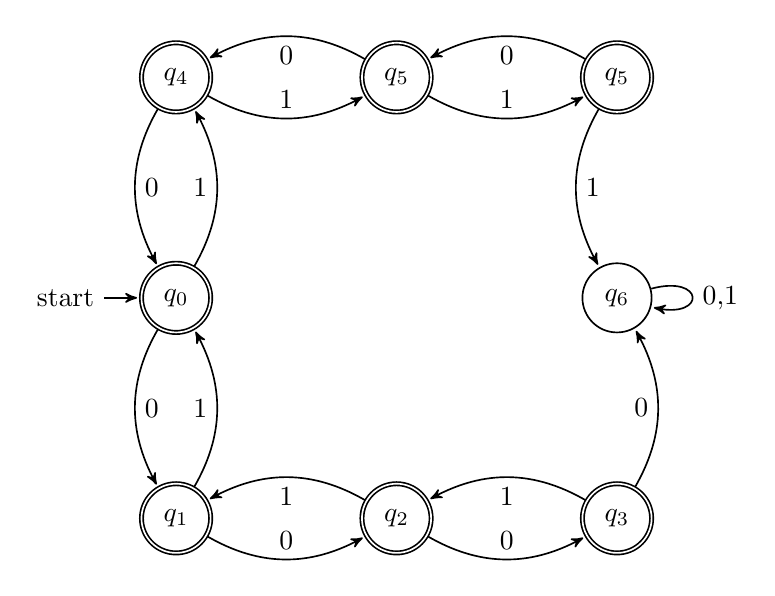
\begin{tikzpicture}[->,>=stealth',shorten >=1pt,auto,node distance=2.8cm,semithick]

\node[initial,state,accepting] (0)                {$q_0$};
\node[state,accepting]         (-1) [below of=0] {$q_1$};
\node[state,accepting]	     (-2)  [right of=-1] {$q_2$};
\node[state,accepting]         (-3) [right of=-2] {$q_3$};
\node[state,accepting]	     (1)  [above of=0] {$q_4$};
\node[state,accepting]         (2) [right of=1] {$q_5$};
\node[state,accepting]         (3) [right of=2] {$q_5$};
\node[state]         (B) [below of=3] {$q_6$};

\path
(0)  edge [bend right] node {0} (-1)
(0)  edge [bend right] node {1} (1)
(1)  edge [bend right] node {0} (0)
(1)  edge [bend right] node {1} (2)
(2)  edge [bend right] node {0} (1)
(2)  edge [bend right] node {1} (3)
(3)  edge [bend right] node {0} (2)
(3)  edge [bend right] node {1} (B)
(-1)  edge [bend right] node {0} (-2)
(-1)  edge [bend right] node {1} (0)
(-2)  edge [bend right] node {0} (-3)
(-2)  edge [bend right] node {1} (-1)
(-3)  edge [bend right] node {0} (B)
(-3)  edge [bend right] node {1} (-2)
(B) edge [loop right] node {0,1} (B)
;
\end{tikzpicture}
\subproblem{}
منظم نیست، فرض کنید منظم است، پس طبق لم تزریق $n$ ای وجود دارد که به ازای هر رشته‌ی با طول بیشتر یا مساوی $n$ مثل $w$ می‌توان $w$ را به صورت $xyz$ نوشت که $|xy| \leq n$ و $|y| \geq 1$ که به ازای هر $k$، $xy^kw$ عضو زبان است.

حال 
$w = 0^n10^n$
را در نظر بگیرید، طبق لم بالا $w=xyz$ ای است که ‌$|xy| \leq n, |y| > 0$ پس $x,y$ تنها از ۰ تشکیل شده اند و باید رشته‌ی 
$xy^2z$
نیز جز زبان باشد که چون اندازه‌ی $y$ حداقل یک است و فقط از ۰ تشکیل شده، در این حالت تعداد صفر‌های قبل از یک حداقل $n+1$ شده‌است، تعداد یک‌ها تغییری نکرده و یک عدد است. تعداد صفر‌های بعد از ۱ نیز تغییری نکرده و $n$ تا باقی مانده است. و چون $n$ نمی‌تواند برابر با حاصل ضرب یک در عددی بزرگتر از $n$ باشد، این رشته عضو زبان نیست که این تناقض است، پس فرض خلف باطل و زبان منظم نیست.
\problem{}
\subproblem{}
غلط است، سمت چپ $\epsilon$ را می‌پذیرد اما سمت راست نه.
\subproblem{}
غلط است، سمت چپ $\epsilon$ را می‌پذیرد اما سمت راست نه.
\subproblem{}
غلط است، سمت چپ $1$ را می‌پذیرد اما سمت راست نه.
\subproblem{}
صحیح است، زیرا از کلاس درس می‌دانیم $(a+b)^* = a^* + b^8$ و همچنین 
$(a^*)^* = a^*$.
و با کمک این دو به سادگی اثبات می‌شود. همچنین زبان این دو برابر با تعداد رشته‌های زوج حرفی است که باهم برابر اند.
\problem{}

\problem{}
\subproblem{}
کافی است مجموعه‌ی 
$S = \{0^n | n \geq 0\}$
را در نظر بگیریم، این مجموعه تمایزگر است زیرا دو عضو دلخواه آن مثل $0^p$ و $0^q$ که $p \neq q$ است در نظر بگیرید، حال رشته‌ی $1^p$ را در نظر بگیرید، $0^p1^p \in L$ اما $0^q1^p \notin L$ پس این دو رشته تمایزپذیرند. پس هر دو عضو از این مجموعه تمایزپذیر بوده و مجموعه تمایزگر است.
\subproblem{}
با برهان خلف مسئله را حل می‌کنیم. فرض کنید
$F = \{w_1, w_2, ..., w_k\}$
باشد و 
$D = (\Sigma, Q, q_0, \delta, F')$
 یک \dfa  با کمتر از $k$ حالت باشد.

تابع $\deltaHat$ برای این \dfa را در نظر بگیرید و حالت‌های زیر را در نظر می‌گیریم،

$$
\deltaHat(q_0, w_1), \deltaHat(q_0, w_2), ..., \deltaHat(q_0, w_k)
$$
چون تعداد حالت‌ها کمتر از $k$ است، پس طبق لانه‌کبوتری $i,j$ ای وجود دارد که 
$\deltaHat(q_0, w_i) = \deltaHat(q_0, w_j)$

اما چون $w_i, w_j$ تمایزپذیرند، $w$ ای وجود دارد که $w_iw \in L(D)$ اما $w_jw \notin L(D)$ (یا برعکس که در این صورت جای $i,j$ را باهم عوض می‌کنیم تا همین حالت پیش آید.)

پس:
$$
\deltaHat(q_0, w_iw) \in F'
$$
اما:
$$
\deltaHat(q_0, w_iw) = \deltaHat(\deltaHat(q_0, w_i), w) = \deltaHat(\deltaHat(q_0, w_j), w) = \deltaHat(q_0, w_jw)
$$
پس:
$$
\deltaHat(q_0, w_jw) \in F' \implies w_jw \in L(D)
$$
که این با 
$w_jw \notin L(D)$
در تناقض است. پس فرض خلف باطل و حکم ثابت است.
\problem{}

\problem{}

\problem{}
درست است،می‌دانیم هر زبان منتاهی ای منظم است، حال 
$\Sigma = \{1\}$
و زبان همه‌ی رشته با طول کمتر یا مساوی $k$ را در نظر بگیرید.ادعا می‌کنیم \dfa برای این زبان باید حداقل $k$ حالت نهایی داشته باشد، فرض کنید تعداد حالت‌نهایی‌ها کمتر از $k$ باشد، در این صورت دو رشته‌‌ی مثل $1^i$ و $1^j$ که $i,j \leq k$ وجود دارند که هر دو به یک حالت نهایی بروند. بدون خدشه به کلید مسئله فرض کنید $i < j$. پس:
$$q = \deltaHat(q_0, 1^j) = \deltaHat(q_0, 1^i) \in F$$
از طرفی:
$$q = \deltaHat(q_0, 1^j) = \deltaHat(\deltaHat(q_0, 1^i), 1^{j-i}) = \deltaHat(q, 1^{j-i})$$
پس به ازای هر $x$،
$$\deltaHat(q, (1^{j-i})^x) = q$$
و در نتیجه 
$$
\deltaHat(q_0, 1^i (1^{j-i})^x) = \deltaHat(\deltaHat(q_0, 1^i), (1^{j-i})^x)
= \deltaHat(q, (1^{j-i})^x) = q \implies 1^i (1^{j-i})^x \in L
$$
اما چون $j-i > 0$، پس $1^i (1^{j-i})^x$ها نامتاهی‌تا هستند پس زبان باید نامتناهی باشد، درحالی که تنها شامل $k$ عضو بود که این تناقض است. پس فرض خلف باطل و حکم ثابت است.
\problem{}


\end{document}
